\section{Applying Design of Computational Experiments to the Problem}
Our first hypothesis on the stated problem posed in the previous chapter is that implementing domain-specific design patterns according to the context variables governing the execution of a software as the most effective way to regulate its performance. However, out goal is to determine how much these variables affect the software performance. 

Given  the nature of the problem guidelines to verify our hypothesis a relevant method is the experimentation. This method usually tries to prove a causal relation between independent variables and a dependent variable. That is, researcher tries to prove that a certain outcome (observation of dependent variable) is obtained when an specific event occurs (specific values of independent variables). However, to use this method implies to design and execute experiments systematically.
%, for example, to prove a hypothesis such as "If there is water in the moon, it will be potable" is impossible to execute experiments.

In this thesis we follow the guidelines presented by \cite{} according to these, the first step to design experiments is to have a good problem understanding. Chapter \ref{cha:modelingProblem} explains in detail the problem. 

Section \ref{sec:variables} presents variables classification and values selected for them. Section \ref{sec:controlandrep} defines how we ensure control and replication of experiments. Because of our experiments are executed in a software environment, we need a case of study which is described in section \ref{sec:sorting}. Based on the selected case of study, the values for the domain-specific design pattern variable are selected in section \ref{sec:selectdesignpatterns}. Finally, section \ref{sec:measureandmonitor} describes how we measure and monitor the variables of experimentation.

\section{Variables}
\label{sec:variables}

Variables represent essential characteristics that define the conditions under which a given event occurs. For example, if a server fails to fulfill a QA of throughput, this situation could be caused by some variables that impact the system such as: (i) number of users (e.g. sudden increase), (ii) hardware components (e.g. electric overload on circuits), (iii) software applications (e.g. to throw an exception), (iv) power energy, and (v) operating system. Significant changes in any of these variables, or in a combination of them could cause the software failure. Therefore, to understand the effect of each variable over the system failure we may need to vary their values. To vary variable values, independent variables should be categorized as (i) controllable,  (ii) uncontrollable, and (iii) Irrelevant, this classification allows to determine if variable values can be defined by the experiment designer (that is, who design experiments to observe how variables affect a target event, in this case the system failure) if the variable only can be observed or if the variable does not affect the target event. Additionally, a target event (or dependent variable) must be defined in order to determine the variables effect over it.

\subsection{Controllable Variables}

In an experiment the controllable variables are those whose values can be configured and modified during the execution of the experiments with the aim of observing how these changes affect the target variables. In this thesis, the domain-specific design patterns variable is categorized as controllable, because as the experiment designers, we can evaluate and select which design patterns can be implemented on the study cases during experiments. Some context variables are also categorized as controllable, for example, the number of available distributed task processors. In the following, we describe the values that selected for each of the controllable variables significant for following the goals of this thesis.

\subsubsection{Selection of the Controllable Context Variables}
\label{sec:contextVariablesControlledSelection}
For the experiments, we selected a subset of variables listed in section \ref{sec:contextVariablesSearch} according to their relevance for our objectives. Additionally, in this section, we select these controllable variables using the following criteria:

\begin{itemize}
	\item The variable must be controllable in the test environment (LIASOn Laboratory).
	\item The variable must be able to be measured accurately (Accuracy).
	\item The variable must be relevant for the selected design patterns (Relevance).
	\item The variable's variation must affect the performance of the software system significantly.
\end{itemize}

Due to the fact that experiments must be executed in a distributed environment, variables that influence the distributed software application performance have more importance. The following are the five selected controllable context variables. 

\begin{itemize}
	\item Number of available distributed task processors.
		This variable can take its values from the set of positive integers. It can be varied according to the experiment designer criteria, in this case, we have 18 available processors. Given that the effect of one processor could be not relevant, we selected only 5 values from the 18 possible values: 1, 2, 4, 8, and 16. 
	\item Number of service requests.
		In many environments this variable can not be controlled, however, in this case, experiment the designer can decide how many service request will be used. To analyze latency, we send one service request at time. Based on latency results and to analyze throughput we send a variable number of service requests, this number should keep the application processing requests for 20 minutes.
	\item Network Bandwidth.
		The test environment allows us only 2 possible values for this variable: 100 MB and 1 GB.
	\item Shared Memory Architecture.
		This variable can take 4 possible values, UMA, NUMA, COMA, NORMA. Implementing each value implies to code, therefore, due to thesis scope we selected only 2 values, UMA and NORMA, which are representative among the whole set.
	\item Communication protocol between components.
		To evaluate how this variable affect system performance (specifically latency and throughput) varying its possible values it is needed to code each value. Therefore, to fulfill the thesis goals without extending it beyond time constraints we select only 3 values, REST, RMI, and ICE.
\end{itemize}

\subsection{Uncontrollable Variables}
Uncontrollable variables influence software performance and measurable target variables, but they cannot be controlled in the experiments. Their configuration during experiments execution can only be monitored. Examples of uncontrollable variable are: environmental temperature, physical CPU cache, and operating system resource management of physical devices.

\subsubsection{Selection of Uncontrollable Context Variables To Monitor}
Similarly as in section \ref{sec:contextVariablesControlledSelection}, in this section we selected a subset of uncontrollable context variables chosen for this thesis scope. This selection uses the same criteria used in the section \ref{sec:contextVariablesControlledSelection}. \\

The following are the two selected uncontrollable context variables.
 
\begin{itemize}
	\item Number of available CPU cores.
		CPU cores used by any software application in its execution is managed by operating system. That is why this is an uncontrollable context variable and we only can monitor how many CPU cores are used during our experiments.
	\item Communication time.
		Time dedicated to communicate 2 distributed processors can not be defined by the experiment designer because it can be affected by many other variables, such as operating systems, network bandwidth, package size, communication protocol, and more determinant variables according to the problem nature. Given that our objective is to determine how context variables affect system performance, we only monitor this uncontrollable context variable.
\end{itemize}

\subsection{Irrelevant Variables}
Due to the scope of this thesis, some variables are classified as irrelevant. Changes on irrelevant variables do not change experiment results between replications. If there are variables that have an impact on experiments and they change the experiments results between an execution and its replication, they will be reclassified or their effect neutralized if possible. One example of these are: If software application does not process a huge amount of data, it does not need a big memory, therefore, memory size could be an irrelevant variable for this application.

\subsection{Target Variables}
These variables are the selected of interest to be measured. That is, this is the dependent variable over the independent variables have an effect. For example: in our thesis dependent variable is performance, specifically its performance factors, such as latency, throughput, capacity, jitter, resource utilization, load balance or success rate (section \ref{subsubsec:performanceFactors}).

\subsubsection{Performance Factors}
\label{subsubsec:performanceFactors}
The choice of performance factors to be measured is based on how many papers use each performance factor (column "Tally" in table \ref{tab:performanceFactors}). We observe that performance factors more relevant in the explored literature are throughput and latency. Therefore, in this thesis we work with both of them. However, each one is treated as an independent variable. That is, we execute independent experiments for each them.
%\section{Control and Experiments Configuration}

\section{Control and Replication}
\label{sec:controlandrep}
The goal of replication is to increase reliability of experiments results, thus, this is an important step in the experiments design. Replication in this thesis depends on performance factors. On the one side, for latency, replication consists in processing 10 files of the same size, but one at a time. On the other side, for throughput, replication consists in executing the same experiment twice, and each experiment consists in processing a number of files enough to maintain a load in the software application during at least 20 minutes.

Additionally, we realize a calibration and control tests to ensure reliability on the experiments environment. We executed the same calibration and control experiments during a whole day. Results of this experiment confirm that no identified environment variables were not affecting experiments. (see section \ref{sec:controlTest}).

\section{Experiment Case of Study: Sorting }
\label{sec:sorting}

The process of arranging elements in specific order is called sorting. Sorting is applied to many in activities of daily life, for example, products can sorted in a supermarket by trademark, files are sorted in an office by name, and mail is sorted in an inbox by arrived date, among others. Many sorting algorithms  have been developed given that this is a classical problem in computer science. There is even a competition whose objective is to sort 1 Petabyte of information in 320 minutes. This suggests that sorting is a relevant problem of analysis. According to section 5.6 of \cite {Miller:2011:PSA:2073661}, sorting a large amount of data always take a substantial amount of computing resources. To improve performance of solutions to this problem there is more than one option: increasing computational resources, developing new processing algorithms more efficient or distributed processing strategy across a series of nodes, among others.

Increasing computational resources can be done vertically (adding resource to only one machine)  or horizontally (taking advantage of several processing machines). The first option is limited by the physical space of the single machine. The second option overrides their limitation, but adds complexity to the single-machine solution. For the strategy, the most suitable should be based on a variation of distributing the sorting solution is not a trivial task, because of the latency introduced by communication could cause that the application performance would be worse than in a non-distributed (monolithic) case. In this thesis, we use an strategy developed by Juan Carlos Mu\~{n}oz (JC sorting strategy). Figure \ref{fig:diagramJCMunoz} shows the deployment diagram for this strategy. The strategy consists of distributing the array to sort according to the nodes level variable. The nodes level refers to the exponent used to calculate how many nodes would be used to sort the input file. This number is calculated in base two, for example, $2 ^{0} = 1 ; 2 ^{1} = 2; 2 ^{2} = 4 ; 2 ^{3} = 8... $, where exponents represents the nodes level (0, 1, 2, ...). Additionally, the nodes level determines how many times the input file would be divided. For example, if the nodes level is zero, the first distributor processes the whole array, that is, the file is not distributed. Another example is, if the nodes level is one, so, two nodes are responsible to sort the file. The first node evaluates if the file must be divided. Due to there is more than one node available to process (according to the nodes level) it divides the input file by half. One of the halves is sent to the bigger son of the node (according to the strategy the nodes are located hierarchically, we called son nodes to the nodes located under  other node and the nodes are biggest according as their amount of son nodes, e.g., Hgrid2 in figure \ref{fig:diagramJCMunoz} is a son of the Hgrid1 and it is its most big son), and another half is assigned to itself. Each time that one division is executed the available nodes level is reduced in one. So, each half of the file is evaluated again in their corresponding node. According to the new nodes level (in this case the new node level is zero) there are not more division to execute, thus, each node processes its half of the input file.

Another example of how the sorting strategy works, for nodes level of three (as in figures \ref{fig:diagramJCMunoz} and \ref{fig:fileProcess}), the first node (Hgrid1) divides the file by half. Same that the before examples. One of the halves is assigned to the most big son of the first node (Hgrid2) and the other half is assigned to the first node. Both nodes evaluate if the file must be divided again according to the new nodes level (currently is 2 because the first division already was executed). As file part of both nodes must be divided again each node divides its file part to the half again. As the most big son of the first node already has work to execute it searches the second most big son node (Hgrid3) to assign one of the halves of file (1/4 of the original file) to him. While the Hgrid2 searches its the most big son node (Hgrid4) to assign one of the halves of file (1/4 of the original file). Now we have four nodes working and the new nodes level is 1. The four nodes evaluate if the file must be divided again according to the new nodes level (currently is 1). Due to the file part of each node must be divided, all search their most big son without work assigned before. In case of Hgrid1 is Hgrid5, for Hgrid2 is Hgrid7, for Hgrid3 is Hgrid6, and finally for Hgrid4 is Hgrid8. Now, the new nodes level is zero. Given that the new nodes level is zero after the 8 nodes evaluate if must be divide their file part they decide that do not need to divide again their file part and they can start to sort. When the nodes level is zero, the file is sorted using the QuickSort algorithm implemented by the Java Array Class. QuickSort is one of the best sorting algorithms \cite{TheTop10Algorithms}, it has an average complexity of O($n log n$) in average and O($ n^{2} $) in the worst performance case. finally, when each file part is sorted (i.e., the nodes level is zero), it is sent to the corresponding father, so each father merges its sorted file part with sorted file parts by its sons. This process is repeated until the first node recover the whole file (i.e., the first father).


\begin{landscape}
	\begin{figure}[p!]
		\centering
		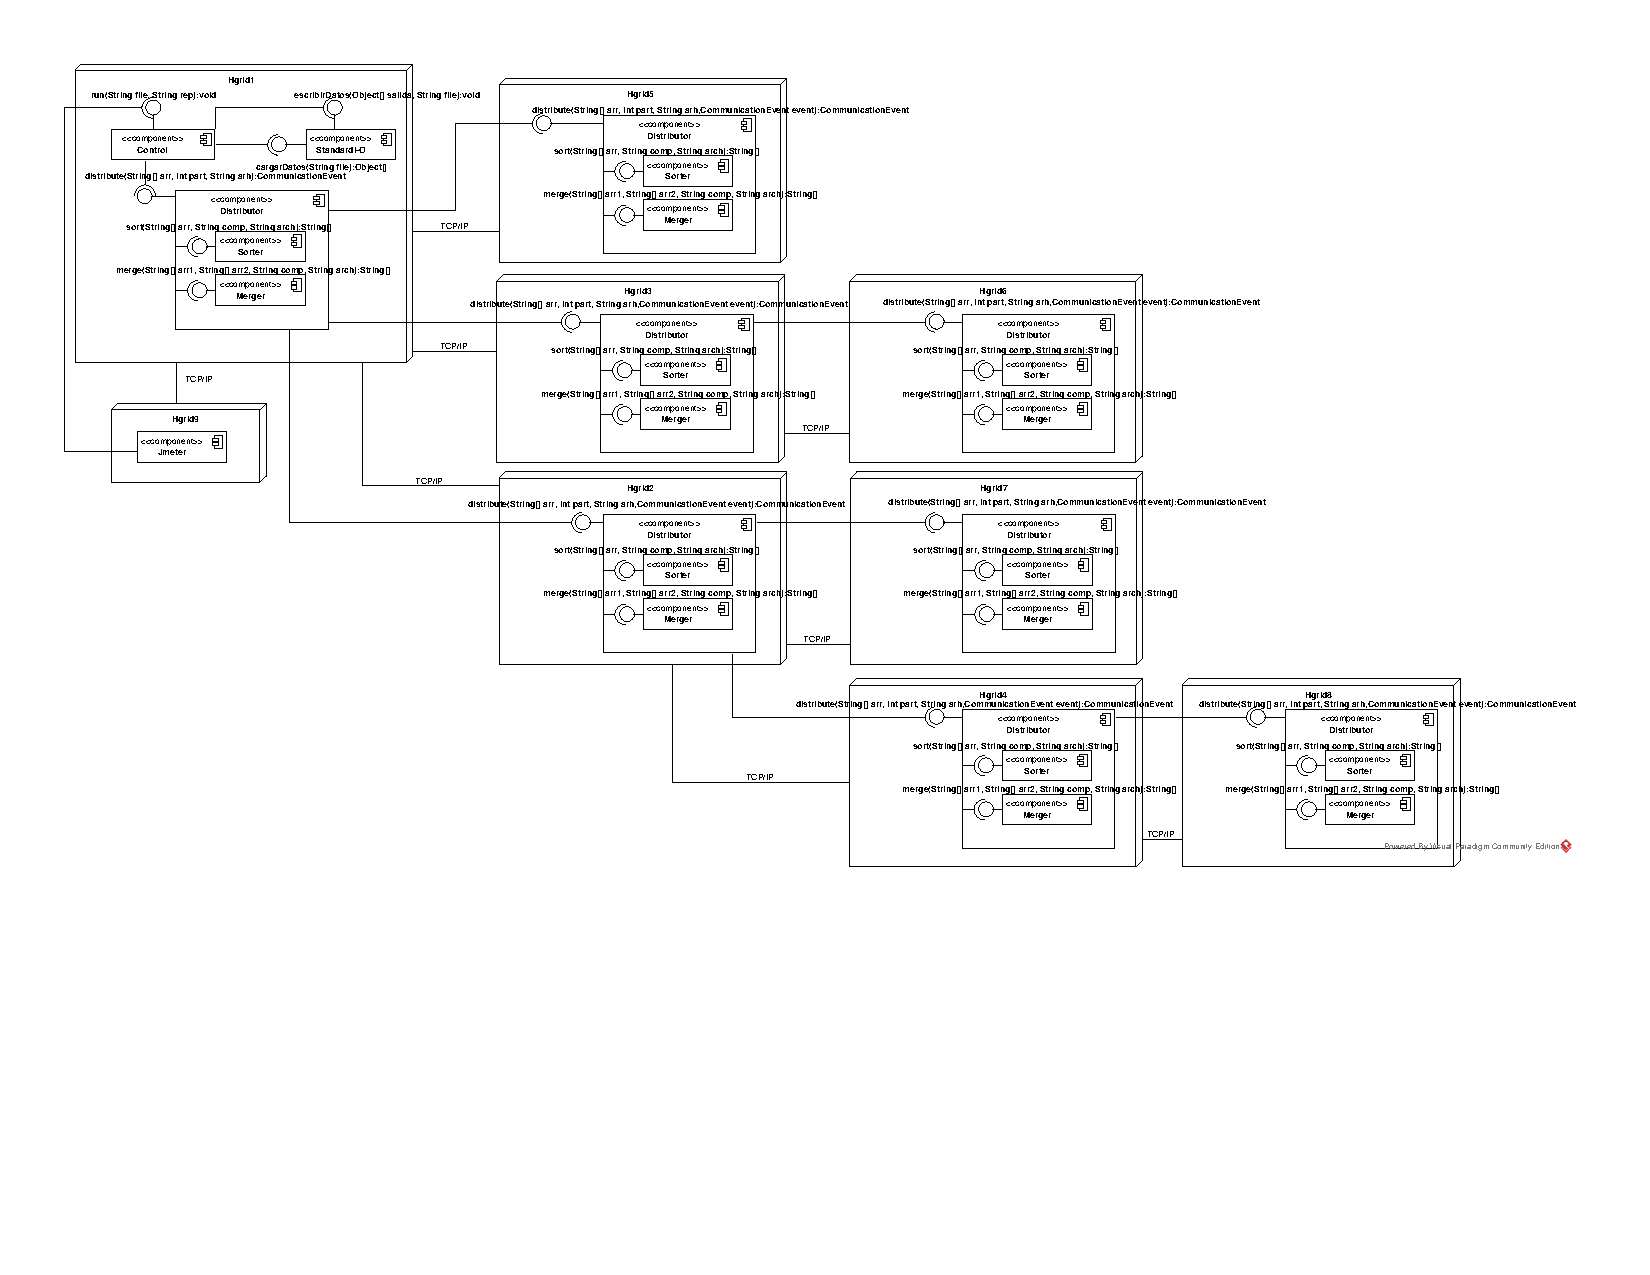
\includegraphics[trim=2cm 6cm 1cm 1cm]{fig/JCMunozDiagrams.pdf}
		\caption{Deployment Diagram - Sorting Strategy}
		\label{fig:diagramJCMunoz}
	\end{figure}	
\end{landscape}

\begin{figure}
	\centering
	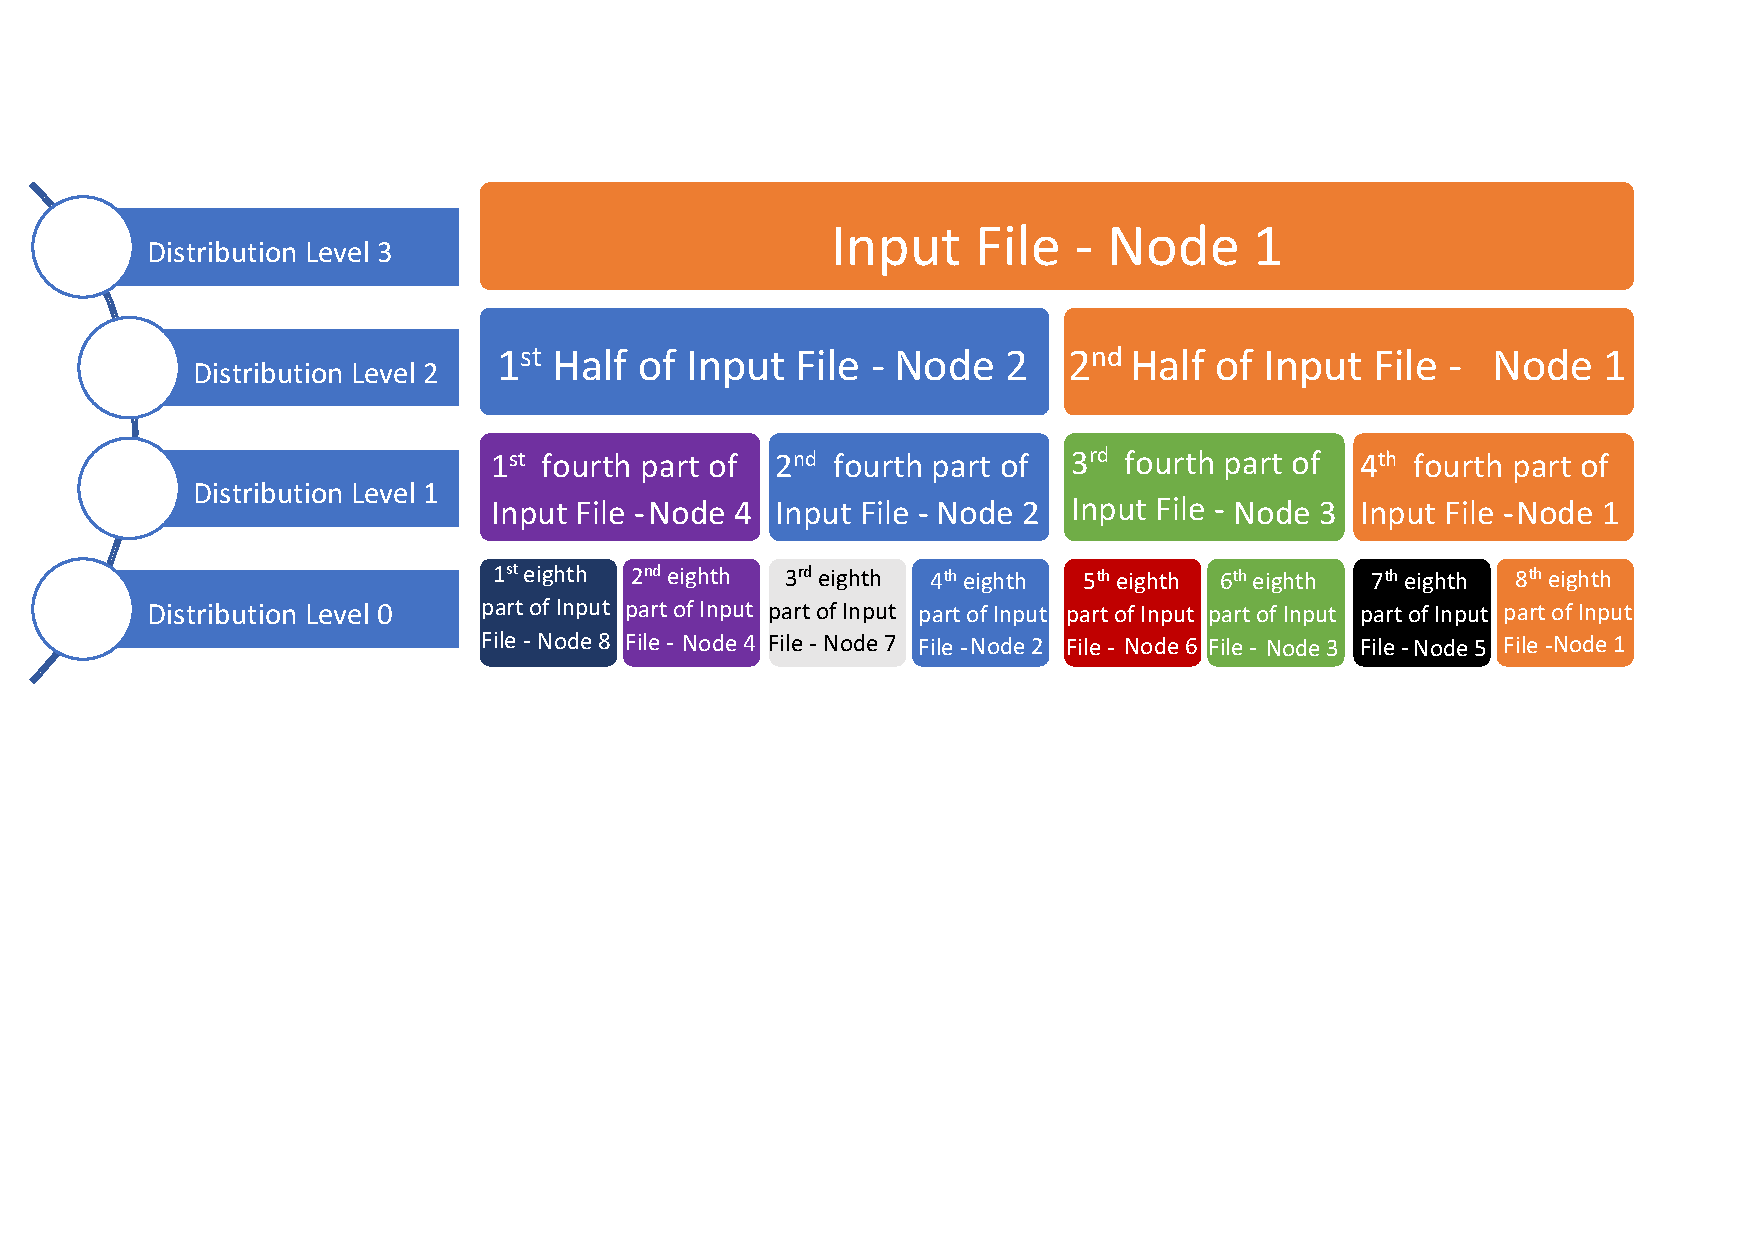
\includegraphics[trim=0cm 8cm 1cm 3cm, scale=0.6]{fig/FileProccess.pdf}
	\caption{File Distribution Process}
	\label{fig:fileProcess}
\end{figure}

\section{Selection of Specific Values of Domain-Specific Design Patterns according to the Case of Study}
\label{sec:selectdesignpatterns}

Not all domain specific performance design patterns are applicable to any problem. Therefore, to achieve the goal of this project we selected domain-specific design patterns to applying our experiments and present a justification of them as exemplars for improving software performance. Our objective is to observe how the selected patterns influence system performance.

\subsection{Applicability of the Domain Specific Design Patterns to the Sorting Problem}

\begin{itemize}
	
	\item Leader / Followers : This pattern is focused on achieving high-performance through multi-threading applications. It processes multiple types of events or service requests concurrently using independents threads (each thread works asynchronously with others). This pattern can be adapted to a distributed software configuration to exploit its benefits. In this thesis we want to leverage this pattern in a distributed environment, therefore we adapt the pattern as follows: (i) the input file to sort is divided in chunks and each chunk is translated as a sorting request, (ii) chunks of the file that must be sorted are stored in an queue to avoid missing data, and (iii) a manager must be implemented being it responsible to send a chunk from the queue to the current leader, (iv) before processing a request, each leader selects a new leader.
	
	\item Half-Synchronous / Half-Asynchronous : This pattern describes in its context two main parts, one asynchronous and one synchronous. The asynchronous part proposes to implement a queue to receive asynchronous requests. The synchronous part proposes to process a task since it starts until its ends.  This pattern is not applicable to the sorting problem because it does not involve asynchronous requests during the sorting process, so,  we would work only with the synchronous part of the process where we process one file at a time. If we want to adapt this pattern we would consume resources unnecessarily due to asynchronism proposed by this pattern. We would propose that in the same way that Leader / Followers was adapted, this pattern could be adapted, however, it implements its own queue to receive the asynchronous requests, thus, increasing latency. Therefore, we discarded it..
	
	\item Master / Workers : This pattern does not consider shared data, it only considers independent tasks. So, it is not possible to exploit this pattern in a distributed environment for the sorting problem, because not all processing nodes are leveraged if the processed file is not shared. However, one of its variants (Separable Dependencies) could be selected because of that variant considers shared data.
	
	\subitem Separable Dependencies Variant : This pattern can be applied to the sorting problem. 
	
	\subitem Geometric Decomposition Variant : This pattern is a variation of Master/Workers. This pattern considers not only independent tasks but also the shared data. To share data, this pattern proposes to divide data into chunks that interact between each other. However, to sort a chunk of a file it is not necessary to have information of other chunks of the file. This means that there is no interaction between data chunks sorters. In the merge phase, chunks could be exploited, however, it will imply to make more than one merge phase. If the sorting case is implemented using more than one merge phase, it can lose performance. That is why this pattern is not exploitable in the sorting case.
	
	\item ThreadPool : This pattern is used by other patterns such as leader / Followers. Thus, its applicability is analyzed in them.
	
	\item Fork / Join : This pattern is applicable because it proposes a way to leverage all available processing units. Since Java version 1.7, it includes an implementation of this pattern. That is the reason why we decided to implement this pattern in two levels. (i) each node implements the Java concurrent library to leverage this pattern in a parallel environment and (ii) this pattern is generalized in a distributed environment.
	
	\item Producer-Consumer : This pattern is applicable to the sorting problem.
	
	\item Random Access Parser : This pattern is applicable to improve XML files processing, thus, this pattern is not applicable in the sorting problem.
	
	\item Map-Reduce : This pattern can be applied to the sorting problem.
	
	\item Sender Released : This pattern is not applicable in this case of study because this pattern has a different main objective to the case of study. This pattern is focused on SOA applications communication to guarantee to deliver messages without affecting performance significantly. In our case, we only have one application (sorting case) and deliverability in the communication among services is not a critic point that justify to implement this pattern. (See section \ref{sec:SLRResults}).
	
	\item The State-Based-Pipeline : This pattern is leveraged when there are more than one processing phase. Even though in the sorting case there are two phases, sort and merge, only the sorting phase can be distributed to leverage the processing units. Because of this, this pattern is not applicable to the sorting problem.
	
	\item Sayl : This pattern proposes a way to leverage idle time of processing units according to task dependencies. However, in this case only the sorting phase can leverage processing units. Therefore it is not possible leverage idle time caused by task dependencies.
	
	\item Reactor : It works as a receptionist, it takes calls (requests) and redirect them to the corresponding addressee (i.e., an instance that can attend the request). In the sorting problem this behavior does not happen, because there is only one kind of request receptor. Therefore, this pattern is not applicable to the sorting problem. 
	
\end{itemize}

\subsection{Selection of the Domain Specific Design Patterns for our Experiments}

Considering to the previous section, we determine that there are 5 domain specific design patterns applicable to the sorting case (i) Leader/Followers, (ii) Separable dependencies, (iii) Fork/Join, (iv) Producer-Consumer, and (v) Map-Reduce. Additionally, our case of study application is based on the strategy proposed by Juan Carlos Mu\~{n}oz (JC Sorting Strategy). Because of this thesis scope we have to reduce the combination and possible values for this variable to three. First, we select the strategy proposed by Juan Carlos Mu\~{n}oz (i.e.,the JC Sorting Strategy) due to this is our base. Second, we use the base strategy to select patterns that could adapt in a better way to it, have in mind comparison among strategies, the pattern Fork/Join has a strategy very similar to ours, so, this has selected. Finally, we select a pattern with a different strategy and among the existing options we select the pattern that we consider could give us better performance, so, we select the Leader/Followers pattern.

\section{Variable Measurement and Monitoring}
\label{sec:measureandmonitor}
Measurement of variables is focused not only on uncontrollable variables in this thesis, we also measure the time of each of the phases of the sorting case of study. The sorting base strategy has five stages to measure: (i) read, (ii) data distribution, (iii) sort, (iv) merge, and (v) write. Communication time is a measurable variable, and also is part of the one stage of the strategy (implied in distribution stage). Finally, the number of available CPU cores variable is measured as the available percentage of each core of each node using the hyperic sigar Java library. However, this measure is not reported when it occurs like the another measurements, it variable needs a monitor that given a specific time pull the measure repetitively until the whole process finished. The another measurements are taken when a specific event occurs (e.g., when a specific component finishes sorting it sends a measurement), but the number of available CPU cores is always changing, therefore it needs a monitor that is constantly taking measurements (in this case, each five seconds, this value does not overload memory with measures and to keep an approximate on the CPU's behavior).

To take measurements, we use the PaSCAni runtime library developed by Miguel Jimenez \cite{6976605}. This library generates the components for a Dynamic Monitoring Infrastructure. The library makes it possible to measure all variables of interest by injecting in source code the code to send measurements to a probe that is responsible for managing (i.e., to receive and to send) measurement information. Additionally, a reporter component was also developed to request and consolidate the probe measurements information. It generates an excel file that contains all measurements taken during an experiment.

\section{Benchmark}
\label{sec:benchmark}
In this section we present a summary of the variables to be analyzed and their values.

\begin{description}
	\item [Available CPUs Cores.] This is an uncontrollable variable, so, for this variable we developed a CPU monitor that reads the CPU usage percentage every five seconds. Each one of the distributed processing nodes in LIASON laboratory has 8 cores (4 physical and 4 logical).
	\item [Available Nodes.] Because of the limited number of processing nodes available in the laboratory and the additional processing constraints introduced by the strategy or design pattern used (e.g., JC sorting strategy increases node in base two, $2^{0}=1 ; 2^{1}=2; 2^{2}=4; 2^{3}=8; 2^{4}=16$). This variable only takes five possible values to keep the experiments comparable.
	\item [Service Requests.] This variable is defined according to the selected performance factors. Latency is observed as one request at a time while throughput is observed as many requests at the same time.
	\item [Bandwidth.] Variation of this variable depends on the configuration options available in the laboratory's hardware, that is, 1 Gbps and 100 Mbps.
	\item [Distributed Memory Structure.] Each distributed memory structure (i.e., UMA, NUMA, COMA, NORMA) implies a code implementation. Given the scope of this thesis we selected only two memory structures. First, we selected NORMA, because this is one option of shared logical memory and distributed physical memory, and additionally, in this structure, unlike NUMA, each processing node is responsible for managing its own data and in the sorting case it allows us processing chunks of input data independently in each processing node. Second, we selected UMA, because it is the only one with shared logical and physical memory, therefore it can take advantage of the NAS device in the laboratory.
	
	On the one hand, implementing NORMA is based on dividing the file that needs to be sorted in equal size chunks according to each strategy or design pattern. Therefore, once processing nodes have their own chunk to sort, they do not need to share information between them. On the other hand, implementing UMA is based on assigning a set of data to be sorted by each processing node. That way, each node only accesses file data that were assigned to it. Implementing UMA uses the BufferedReader Java implementation and its skip method to read just the assigned data to each node.
	
	\item [Communication Protocol.] There are several frameworks, standards, platforms, and middleware developed to support distributed computation, and each one implies a different code implementation. Due to the scope of this thesis we selected only two middleware/framework that allowed us to use three communication protocols. 
	
	The first, selected middleware/framework is FraSCAti, which provides three kind of communication protocols, (i) Remote Method Invocation (RMI), (ii) Representational state transfer (REST), and (iii) Simple Object Access Protocol (SOAP). Currently, these protocols are the most used for distributed computation. However, we must select only two protocols due to time constraints. We selected the option of WebService communication protocol (REST or SOAP) and RMI. According to \cite{kumari2015performance} in general REST has better response times and throughput than SOAP, thus, we select REST as the WebService option.
	
	The second selected middleware/framework is ICE, according to \cite{articleIce}, Ice has the best performance when it was compared with the other options. Ice is a Remote procedure call (RPC) framework and it has its own Interface description language (IDL) named Slice. Therefore, our third selected communication protocol is RPC-Slice.
	
	\item [Communication Time.] This variable can only be monitored and measured and it depends mostly on the nature of the solution strategy used to solve the problem of interest, in this case the sorting problem.
	\item [Design Patterns.] Among variations of design patterns the first is the JC sorting strategy proposed by Juan Carlos Mu\~{n}oz, this strategy was described in section \ref{sec:sorting}. Despite of this strategy seems as an efficient way to leverage distribution in the context of the sorting problem, we think that it had an improvement opportunity. Therefore, we proposed a variation of this strategy where merge component is centralized. Given that each variation of this variable implies code implementation and we have two base strategies, we selected only two additional design pattern variations (i) Fork-Join and (ii) Leader-Followers (See section \ref{subsubsec:selectdesignpatterns}). \\
	During Fork-Join implementation we find a library with Java fork-join implementation \cite{lea2000javae} and we decided to add a new variation using this library.
	\item [Performance Factors.] In this thesis we selected Latency and Throughput as performance factors to be measured and characterized (See section \ref{subsubsec:performanceFactors}).
	\item [File Size.] (Problem Size) This variable requires calibration experiments to define its possible values. The calibration experiment consists in measuring the time to sort  different file sizes using one and two  processing nodes until finding the minimum file size where using two processing nodes has better performance than using one processing node. To identify this minimum value we increased the file size in 200.000 lines each time and this calibration experiment is executed for all design pattern variation. We found that minimum file size for experiments is 1'800.000 lines (the minimum common file size for all design pattern variation). We propose increasing 400.000 lines at a time until reaching 9'800.000 lines to execute our experiments. The minimum file size found is the point in which distribution environment can be leveraged. Table \ref{tab:mimfileSizeEx} shows results of this calibration experiment.
\end{description}

Table \ref{tab:benchmarks} summarizes experiments variations to be performed, that is, our design for the experiments.

\begin{table}[]
	\centering
	\caption{Benchmark Consolidation}
	\label{tab:benchmarks}
	\resizebox{\textwidth}{!}{%
		\begin{tabular}{|c|c|c|c|c|}
			\hline
			\textbf{Id} & \textbf{\begin{tabular}[c]{@{}c@{}}Context\\   Variables\end{tabular}} & \textbf{Possible Values}                                                                                                                                                                                                                            & \textbf{Controllable} & \textbf{\begin{tabular}[c]{@{}c@{}}Possible\\   Variations\end{tabular}} \\ \hline
			1           & \begin{tabular}[c]{@{}c@{}}Available\\ CPU Cores\end{tabular}              & {[}1-8{]}                                                                                                                                                                                                                                           & No                    & NA                                                                        \\ \hline
			2           & \begin{tabular}[c]{@{}c@{}}Available Distributed\\ Processing Nodes\end{tabular}             & {[}1, 2, 4, 8,16{]}                                                                                                                                                                                                                                 & Yes                    & 5                                                                        \\ \hline
			3           & \begin{tabular}[c]{@{}c@{}}Service\\ Requests\end{tabular}             & \begin{tabular}[c]{@{}c@{}}1. 10 files, one file at a time for latency.\\ 2. Amount of files needed to maintain load \\ during 20 minutes for throughput.\end{tabular}                                                                                       & Yes                    & 2                                                                        \\ \hline
			4           & Bandwidth                                                              & {[}100 Mbps - 1 Gbps{]}                                                                                                                                                                                                                                   & Yes                    & 2                                                                        \\ \hline
			5           & \begin{tabular}[c]{@{}c@{}}Memory\\ Structure\end{tabular}             & UMA, NORMA                                                                                                                                                                                                                                          & Yes                    & 2                                                                        \\ \hline
			6           & \begin{tabular}[c]{@{}c@{}}Communication\\   Protocol\end{tabular}     & REST, Slice, RMI                                                                                                                                                                                                                                    & Yes                    & 3                                                                        \\ \hline
			7           & \begin{tabular}[c]{@{}c@{}}Communication\\ Time\end{tabular}           & {[}0-*{]} (Continuous)                                                                                                                                                                                                                                          & No                    & NA                                                                        \\ \hline
			8           & \begin{tabular}[c]{@{}c@{}}Design Patterns\\ and Strategies Variation\end{tabular}  & \begin{tabular}[c]{@{}c@{}}1. JC Sorting Strategy.\\     2. JC Sorting Strategy Variation \\ (separated merger).\\     3. Fork/Join Java library.\\     4. Fork/Join Java library and\\  Distributed Fork/Join.\\     5. Leader-Followers.\end{tabular} & Yes                    & 5                                                                        \\ \hline
			9           & \begin{tabular}[c]{@{}c@{}}Performance\\ Factors\end{tabular}          & Latency, Throughput                                                                                                                                                                                                                                 & Yes                    & 2                                                                        \\ \hline
			10          & File Size                                                              & \begin{tabular}[c]{@{}c@{}}From 1'800,000 To 9'800,000 \\ with increasing steps of 400,000\end{tabular}                                                                                                                                                   & Yes                    & 21                                                                       \\ \hline
		\end{tabular} %
	}
\end{table}

\section{Chapter Summary}
In this chapter, we follow step by step how we design our solution proposal. We started proposing computational experiments as a possible solution for our problem, so, we define a design of experiments applied it. However, proposing the design was not a trivial task, we first identify the involved variables in the problem. After, we define strategies of control and replication to assurance experiments' reliability. Next, we select a case of study over which we apply the domain-specific design patterns to execute different experiment configurations and based on it we could evaluate the quantitative impact that patterns for performance have on the system, in this case, we selected sorting as our study case. Due to the thesis scope, we can not execute experiments about all domain-specific design patterns that could be applied to our study case, so, we had to select which we consider as the more relevant according to their impact over our problem and their applicability over our study case. Later, we define how we take the measurements and how we monitor the studied variables. Finally, we resume all decisions that we toke in the benchmark section where we present the design of the consolidate experiment.